The resulting FogGuru deployment diagram is presented in Figure~\ref{fig:deployment}. It shows which components got deployed on which node, their roles and interfaces. To make it run, three main challenges had to be overcome.

\paragraph*{Creating the swarm nodes}
Docker Swarm can run on multiple resource-constrained devices such as Raspberry Pi. Using Docker CLI commands, it is possible to create cluster nodes. In our case, one node functions as a Swarm Manager node, others as Workers. The configuration deployed consists of 5 Raspberry Pis, interlinked locally with a docker swarm network.

\paragraph*{Getting Apache Flink to run on Raspberry Pi}
Apache Flink runtime consists of 2 types of processes: At least one Job Manager coordinates the distributed execution and Task Managers (workers) execute tasks and exchange data streams. The design is to run Job and Task managers on different swarm cluster nodes. To run Flink on Raspberry Pi, we configured the Job Manager heap-memory size to 512MB, and the Task Manager heap memory size to 256MB. Also, we enabled Flink's built-in monitoring and metrics system to allow developers to monitor their Flink jobs. Flink Metrics were queried via REST API, which used with Prometheus and Grafana for monitoring and visualizing.

We used dockers buildx feature to create custom Apache Flink docker image for ARMv7 processor and hosted the image on DockerHub public repository\footnote{https://hub.docker.com/repository/docker/digitaljazz/flink-1.8.0-armv7}.

\paragraph*{Building the software}
Docker Stack is included in the Docker Engine. We used Docker Stack to compose the services running on the cluster. Also, we designed the service placement: Which services should run on which nodes, how many replications, which services should connect using which network etc., and wrapped it in a YAML script for 1 click deployment\footnote{https://flink-fog-cluster.readthedocs.io/en/latest}. The advantage of this method is that application developers can easily modify its internal services, and they only have to push a JAR file to deploy a fog application.

\begin{figure}[htbp]
\centerline{
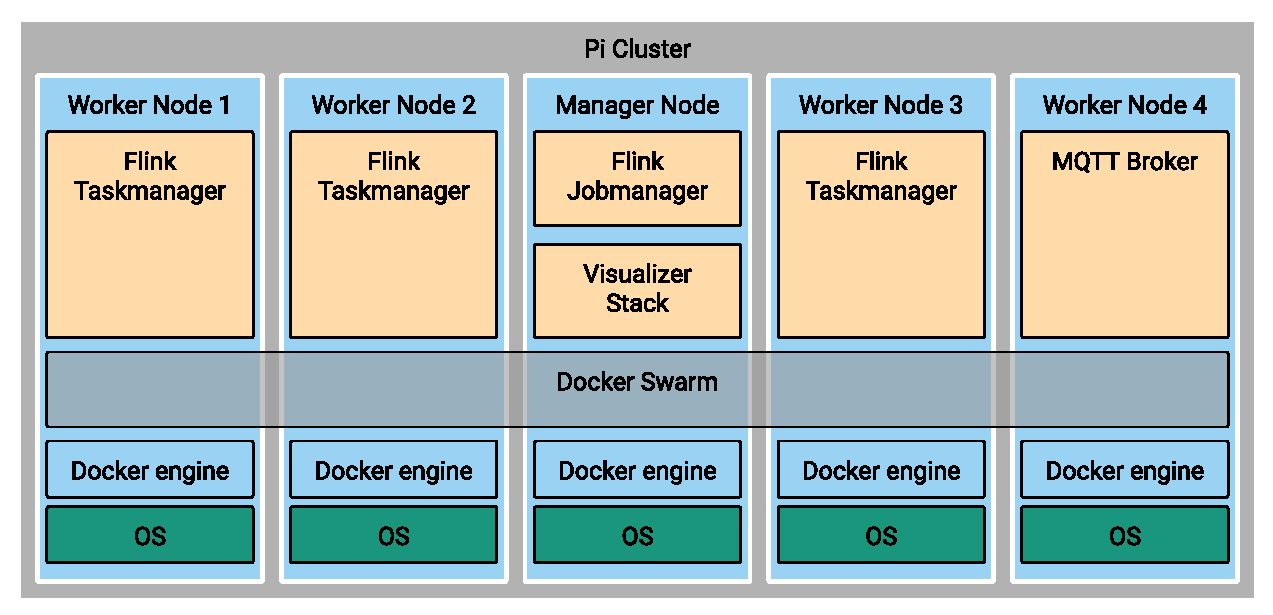
\includegraphics[width=1\linewidth]{figures/fog_platform.pdf}}
\caption{FogGuru: deployment view.}
\label{fig:deployment}
\end{figure}
